\documentclass{article}
\usepackage[utf8]{inputenc}

\title{EE2703: Assignment 7}
\author{Yogesh Agarwala \\ EE19B130}
\date{April 25, 2021}


\usepackage{natbib}
\usepackage{graphicx}
\usepackage{amsmath}
\usepackage{listings}

\begin{document}

\maketitle

\section{Introduction}
This week's assignment involves the analysis of filters using laplace transforms. Python's symbolic solving library, sympy is a tool we use in the process to handle our requirements in solving Modified Nodal Analysis  equations. Besides this the library also includes useful classes to handle the simulation and response to inputs.

Coupled with scipy's signal module, we are able to analyse both High pass and low pass filters, both second order, realised using a single op amp



\section{Assignment}
\subsection{Low pass Filter}
\begin{figure}[h!]
	\centering
	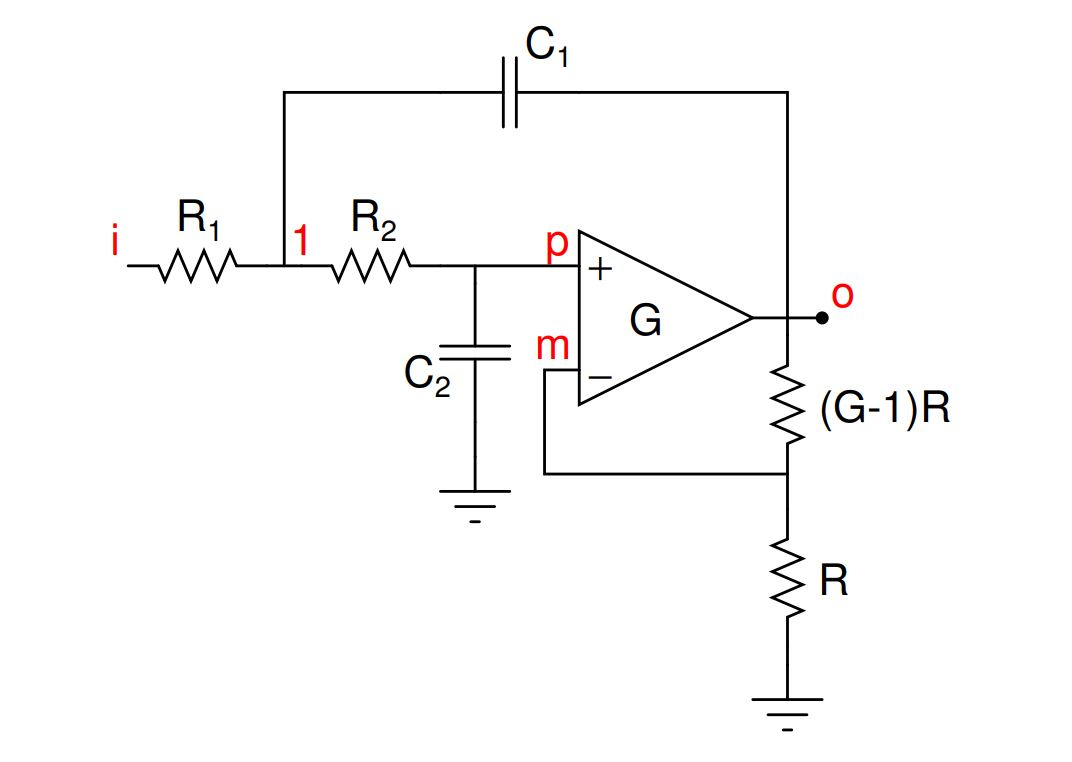
\includegraphics[scale=0.4]{lowpass.jpg}
	\caption{A Lowpass Filter}
	\label{fig:A Lowpass Filter}
\end{figure}

\clearpage

The low pass filter we use gives the following matrix after simplification of Modified Nodal Equations.
\\
$\begin{bmatrix}
    0   & 0 & 1  & -1/G \\
    \frac{-1}{sR_2C_2}  & 1 & 0 & 0\\
    0  & -G & G & 1 \\
    \frac{-1}{R_1} - \frac{1}{R_2} - s*C_1 & \frac{1}{R_2} & 0 & sC_1
\end{bmatrix}$
$\begin{bmatrix}
    V_1\\
    V_p\\
    V_m \\
    V_o
\end{bmatrix}$
=
$\begin{bmatrix}
    0 \\
    0 \\
    0 \\
    \frac{-V_i(s)}{R_1} \\
    
\end{bmatrix}$
\lstset{language=Python}
\lstset{frame=lines}
\lstset{label={lst:code_direct}}
\lstset{basicstyle=\footnotesize}
\newline
\newline


The magnitude bode plot for the filter looks like:
\begin{figure}[h!]
\centering
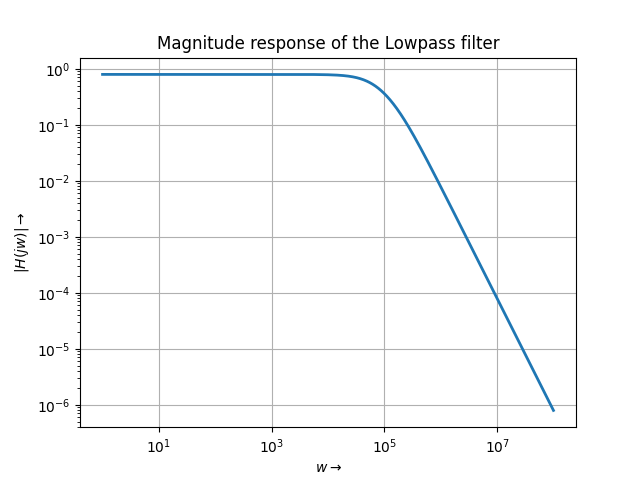
\includegraphics[scale=0.5]{Figure_1.png}
\caption{Lowpass filter magnitude response}
\label{fig:Lowpass filter magnitude response}
\end{figure}

\begin{figure}[h!]
	\centering
	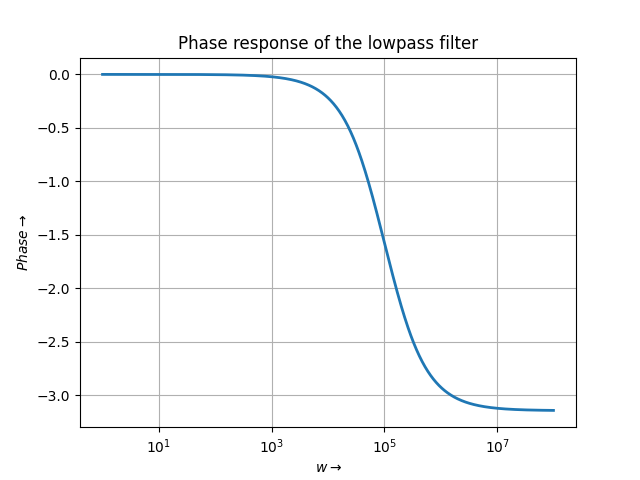
\includegraphics[scale=0.5]{Figure_2.png}
	\caption{Lowpass filter phase response}
	\label{fig:Lowpass filter phase response}
\end{figure}

\clearpage

The unit step response for the low pass filter:


\begin{figure}[h!]
	\centering
	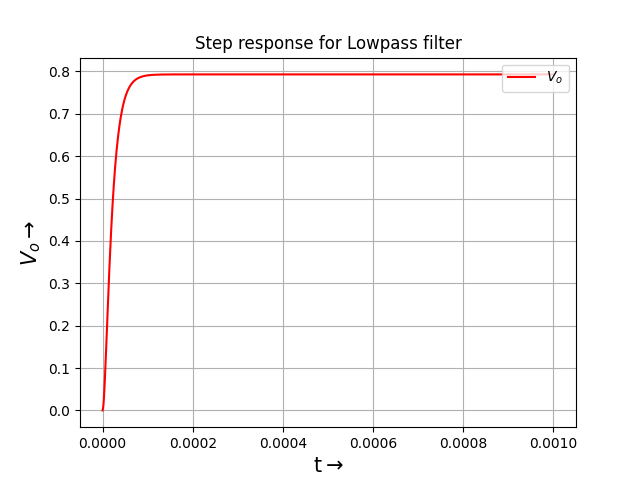
\includegraphics[scale=0.55]{Figure_3}
	\caption{Step response for Lowpass filter}
	\label{fig:Step response for Lowpass filter}
\end{figure}


\subsection{Response of Lowpass Filter to mixed freq sinusoid}

\begin{figure}[h!]
	\centering
	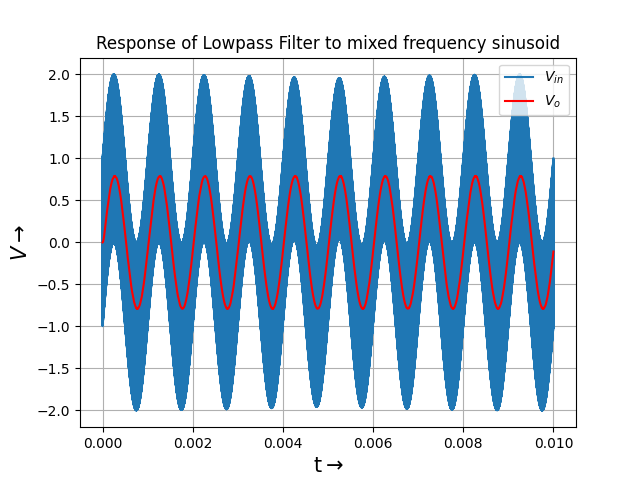
\includegraphics[scale=0.55]{Figure_4}
	\caption{Response of Lowpass Filter to mixed freq sinusoid}
	\label{fig:Response of Lowpass Filter to mixed freq sinusoid}
\end{figure}
We notice that the high frequency part has been attenuated.



\clearpage
\subsection{High pass Filter}

The high pass filter we use gives the following matrix after simplification of Modified Nodal Equations.
\newline

$\begin{bmatrix}
    0   & -1 & 0  & 1/G \\
    \frac{s*C_2*R_3}{1+s*C_2*R_3}  & 0 & -1 & 0\\
    0  & G & -G & 1 \\
    -s*C_2 - \frac{1}{R_1} - s*C_1 & 0 & s*C_2 & \frac{1}{R_1}
\end{bmatrix}$
$\begin{bmatrix}
    V_1\\
    V_p\\
    V_m \\
    V_o
\end{bmatrix}$
=
$\begin{bmatrix}
    0 \\
    0 \\
    0 \\
    -V_i(s)*s*C_1 \\
    
\end{bmatrix}$
\newline
\newline


The magnitude bode plot for the filter looks like:
\begin{figure}[h!]
\centering
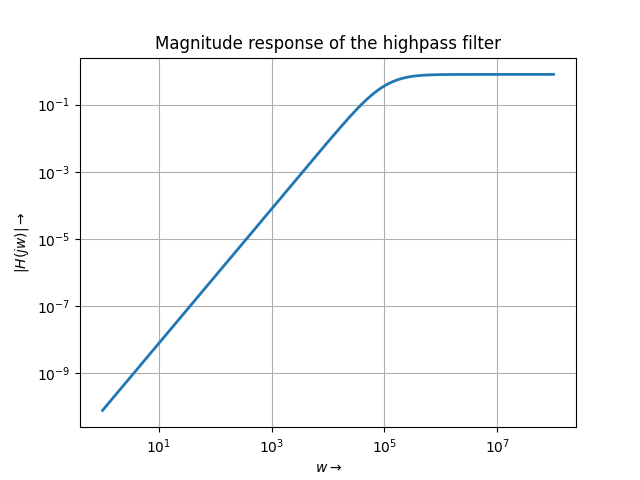
\includegraphics[scale=0.45]{Figure_5.png}
\caption{High pass filter magnitude response}
\label{fig:High pass filter magnitude response}
\end{figure}
\begin{figure}[h!]
	\centering
	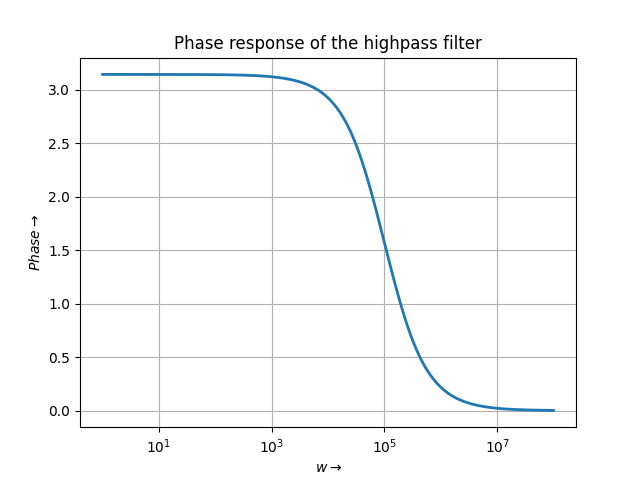
\includegraphics[scale=0.45]{Figure_6.png}
	\caption{High pass filter phase response}
	\label{fig:High pass filter phase response}
\end{figure}



\clearpage


\subsection{Response of Highpass filter to a damped sinusoid}

\subsubsection{Low frequency damped sinusoid}
The Low frequency damping sinusoid is given by:
\begin{equation}
	f(t) = sin(2\pi10^3t)*e^{-1000t}
\end{equation}
It is expected that it will be fully attenuated by the high pass filter while it will pass through the Low pass filter with almost no change.
\begin{figure}[h!]
	\centering
	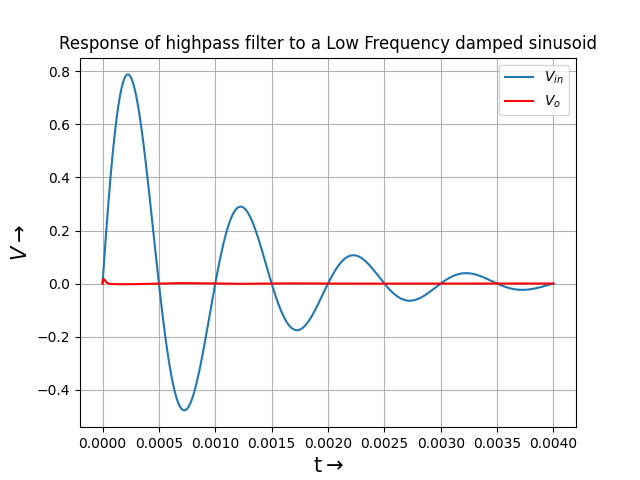
\includegraphics[scale=0.6]{Figure_7.png}
	\caption{Response of Highpass filter to a Low Frequency damped sinusoid}
	\label{fig:Response of Highpass filter to a Low Frequency damped sinusoid}
\end{figure}

The high pass filter responds by quickly attenuating the input. Notice that the time scales show that the high pass filter response is orders of magnitudes faster than the low pass response. This is because the input frequency is below the cutoff frequency, so the output goes to $0$ very fast.

\clearpage

\subsubsection{High frequency damped sinusoid}
The High frequency damping sinusoid is given by:
\begin{equation}
    f(t) = sin(2\pi10^6t)*e^{-100000t}
\end{equation}
It is expected that it will be fully attenuated by the Low passs filter while it will pass through the high pass filter with almost no change.
\begin{figure}[h!]
\centering
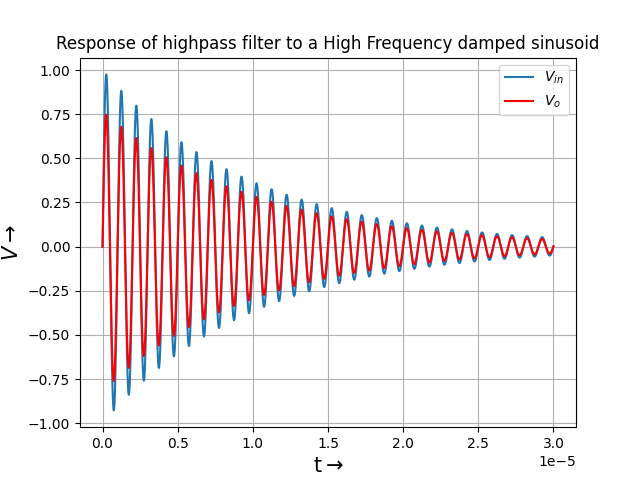
\includegraphics[scale=0.6]{Figure_8.png}
\caption{Response of Highpass filter to a High Frequency damped sinusoid}
\label{fig:System Response with Decay = 0.05}
\end{figure}

\clearpage

\subsection{Response of Highpass filter to a unit step function}
The unit step response, as expected is high at t=0 when there is an abrupt change in the input. Since there is no other change at large time values outside the neighbourhood of 0, the Fourier transform of the unit step has high values near 0 frequency, which the high pass filter attenuates.

\begin{figure}[h!]
\centering
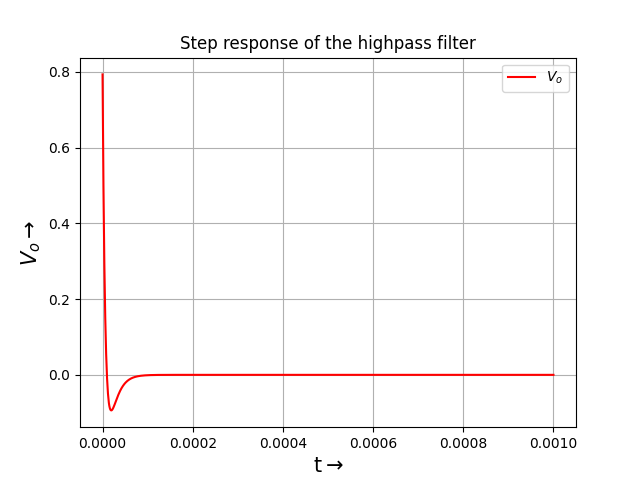
\includegraphics[scale=0.6]{Figure_9}
\caption{Step response of highpass filter}
\label{fig:System Response with Decay = 0.05}
\end{figure}

\section{Conclusion}
\begin{itemize}
\item Output response of Lowpass Filter to mixed frequency sinusoid shows that the Lowpass filter passes only the low frequency component and almost completely attenuates
the high frequency part, as expected.


\item From the step-response, of the low pass filter, it is seen that, at steady
state, output is a constant value (at a very low attenuation). This is because, low pass filter will pass DC signals , and at time t much greater 0,
step input is a DC input. At t = 0, though the rise is gradual, as the capacitors themselves take time to charge, and once they have done, the output
becomes DC.

\item Output response of Highpass filter to a damped sinusoid shows that it attenuates the low frequency damped sinusoid, while allow the high frequency damped sinusoids such as $10^6$ Hz as they are above the
cut-off frequency. Also note that the change in
the exponential would only affect the rate at which the sinusoid amplitude
decays to zero.


\item From the step-response of the high pass filter, it is seen that at t much
greater than 0, output is 0. This is because, at these instants, input is a
DC value and the high pass filter will attenuate this, and thus output will
be almost 0. At t = 0, though, there is a peak for the output. This is because, at this point of discontinuity in the input, as seen from the frequency
domain, a lot of high frequency components would be there, hence these
would be passed, and so, an output is observed only at this point. 

\end{itemize}
\end{document}
